\documentclass[12pt,oneside]{book}

%%%%%%%%%%%%%%%%%%%%%%%%%%%%%%%%%%%%%%%%%%%%%%%%%%%%%%%%%%%%%%%%%%%%%%%%%%%%%%%%%%%%%%%%%%%%%%%%%%%
%                                                                                                 %
% The mathematical style of these documents follows                                               %
%                                                                                                 %
% A. Thompson and B.N. Taylor. The NIST Guide for the Use of the International System of Units.   %
%    NIST Special Publication 881, 2008.                                                          %
%                                                                                                 %
% http://www.nist.gov/pml/pubs/sp811/index.cfm                                                    %
%                                                                                                 %
%%%%%%%%%%%%%%%%%%%%%%%%%%%%%%%%%%%%%%%%%%%%%%%%%%%%%%%%%%%%%%%%%%%%%%%%%%%%%%%%%%%%%%%%%%%%%%%%%%%

% $Date: 2013-11-26 10:43:59 -0500 (Tue, 26 Nov 2013) $
% $Revision: 17538 $
% $Author: gforney $

%%%%%%%%%%%%%%%%%%%%%%%%%%%%%%%%%%%%%%%%%%%%%%%%%%%%%%%%%%%%%%%%%%%%%%%%%%%%%%%%%%%%%%%%%%%%%%%%%%%
%                                                                                                 %
% The mathematical style of these documents follows                                               %
%                                                                                                 %
% A. Thompson and B.N. Taylor. The NIST Guide for the Use of the International System of Units.   %
%    NIST Special Publication 881, 2008.                                                          %
%                                                                                                 %
% http://www.nist.gov/pml/pubs/sp811/index.cfm                                                    %
%                                                                                                 %
%%%%%%%%%%%%%%%%%%%%%%%%%%%%%%%%%%%%%%%%%%%%%%%%%%%%%%%%%%%%%%%%%%%%%%%%%%%%%%%%%%%%%%%%%%%%%%%%%%%

% Packages which force the use of better TeX coding
% Mostly from http://tex.stackexchange.com/q/19264
%%\RequirePackage[l2tabu, orthodox]{nag}
%%\usepackage{fixltx2e}
%\usepackage{isomath} % Disabled for the moment because it changes the syntax for bold and roman Greek math symbols
%%\usepackage[all,warning]{onlyamsmath}
%\usepackage{strict} % Commented out for now because it is uncommon. A copy of style.sty is in Manuals/LaTeX_Style_Files/.

\usepackage{times,mathptmx}
\usepackage[pdftex]{graphicx}
\usepackage{tabularx,ragged2e,booktabs,caption}
\usepackage{multirow}
\usepackage{pdfsync}
\usepackage{tikz}
\usepackage{pgfplots}
%\pgfplotsset{compat=1.7}
\usepackage{tocloft}
\usepackage{color}
\usepackage{amsmath}
\definecolor{linknavy}{rgb}{0,0,0.50196}
\definecolor{linkred}{rgb}{1,0,0}
\definecolor{linkblue}{rgb}{0,0,1}
\usepackage{float}
\usepackage{caption}
\usepackage{graphpap}
\usepackage{rotating}
\usepackage{graphicx}
\usepackage{geometry}
\usepackage{relsize}
\usepackage{longtable}
\usepackage{lscape}
\usepackage{amssymb}
\usepackage{makeidx} % Create index at end of document
\usepackage[nottoc,notlof,notlot]{tocbibind} % Put the bibliography and index in the ToC
\usepackage{lastpage} % Automatic last page number reference.
\usepackage[T1]{fontenc}
\usepackage{enumerate}
\usepackage{upquote}
\usepackage{moreverb}
\usepackage{xfrac}
\usepackage{cite}

\newcommand{\nopart}{\expandafter\def\csname Parent-1\endcsname{}} % To fix table of contents in pdf.
\newcommand{\ct}{\tt\small} % eventually will be deprecated due to http://www.tex.ac.uk/cgi-bin/texfaq2html?label=2letterfontcmd
\newcommand{\textct}[1]{\texttt{\small #1}}

\usepackage{tocstyle} % Fix table of contents sections from overlapping section titles
\usetocstyle{standard}
\usepackage{siunitx}
\sisetup{
    detect-all = true,
    input-decimal-markers = {.},
    input-ignore = {,},
    inter-unit-product = \ensuremath{{}\cdot{}},
    multi-part-units = repeat,
    number-unit-product = \text{~},
    per-mode = fraction,
    separate-uncertainty = true,
}

\usepackage{listings}
\usepackage{textcomp}
\definecolor{lbcolor}{rgb}{0.96,0.96,0.96}
\lstset{
    %backgroundcolor=\color{lbcolor},
    tabsize=4,
    rulecolor=,
    language=Fortran,
        basicstyle=\footnotesize\ttfamily,
        upquote=true,
        aboveskip={\baselineskip},
        belowskip={\baselineskip},
        columns=fixed,
        extendedchars=true,
        breaklines=true,
        breakatwhitespace=true,
        frame=none,
        showtabs=false,
        showspaces=false,
        showstringspaces=false,
        identifierstyle=\ttfamily,
        keywordstyle=\color[rgb]{0,0,0},
        commentstyle=\color[rgb]{0,0,0},
        stringstyle=\color[rgb]{0,0,0},
}

\usepackage[pdftex,
        colorlinks=true,
        urlcolor=linkblue,     % \href{...}{...} external (URL)
        citecolor=linkred,     % citation number colors
        linkcolor=linknavy,    % \ref{...} and \pageref{...}
        pdfproducer={pdflatex},
        pdfpagemode=UseNone,
        bookmarksopen=true,
        plainpages=false,
        verbose]{hyperref}

% The Following commented code makes the ``Draft'' watermark on each page.
%\usepackage{eso-pic}
%\usepackage{type1cm}
%\makeatletter
%   \AddToShipoutPicture{
%     \setlength{\@tempdimb}{.5\paperwidth}
%     \setlength{\@tempdimc}{.5\paperheight}
%     \setlength{\unitlength}{1pt}
%     \put(\strip@pt\@tempdimb,\strip@pt\@tempdimc){
%     \makebox(0,0){\rotatebox{45}{\textcolor[gray]{0.75}{\fontsize{8cm}\selectfont{RC6}}}}}
% }
%\makeatother

\setlength{\textwidth}{6.5in}
\setlength{\textheight}{9.0in}
\setlength{\topmargin}{0.in}
\setlength{\headheight}{0.pt}
\setlength{\headsep}{0.in}
\setlength{\parindent}{0.25in}
\setlength{\oddsidemargin}{0.0in}
\setlength{\evensidemargin}{0.0in}
\setlength{\leftmargini}{\parindent} % Controls the indenting of the "bullets" in a list
\setlength{\cftsecnumwidth}{0.45in}
\setlength{\cftsubsecnumwidth}{0.5in}
\setlength{\cftfignumwidth}{0.45in}
\setlength{\cfttabnumwidth}{0.45in}

\newcommand{\titlesigs}
{
\small
\flushright{U.S. Department of Commerce \\
{\em Penny Pritzker, Secretary} \\
\hspace{1in} \\
National Institute of Standards and Technology \\
{\em Willie May, Under Secretary of Commerce for Standards and Technology and Acting Director} }
}

% commands to use for "official" cover and title pages
% see smokeview verification guide to see how they are used

\newcommand{\headerA}[1]{
\flushright{
\fontsize{20}{24}\selectfont
\bf{NIST Special Publication #1}}
}

\newcommand{\headerB}[1]{
\flushright{
\fontsize{28}{33.6}\selectfont
\bf{#1}
}
}

\newcommand{\headerC}[1]{
\vspace{.5in}
\flushright{\fontsize{14}{16.8}\selectfont
#1}
}

\frenchspacing

\newcommand{\dod}[2]{\frac{\partial #1}{\partial #2}}
\newcommand{\DoD}[2]{\frac{\mathrm{D} #1}{\mathrm{D} #2}}
\newcommand{\dsods}[2]{\frac{\partial^2 #1}{\partial #2^2}}
\renewcommand{\d}{\,\mathrm{d}}
\newcommand{\dx}{\delta x}
\newcommand{\dy}{\delta y}
\newcommand{\dz}{\delta z}
\newcommand{\degF}{$^\circ$F}
\newcommand{\degC}{$^\circ$C}
\newcommand{\x}{x}
\newcommand{\y}{y}
\newcommand{\z}{z}
\newcommand{\dt}{\delta t}
\newcommand{\dn}{\delta n}
\newcommand{\cH}{H}
\newcommand{\hu}{u}
\newcommand{\hv}{v}
\newcommand{\hw}{w}
\newcommand{\la}{\lambda}
\newcommand{\bO}{{\Omega}}
\newcommand{\bo}{{\mathbf{\omega}}}
\newcommand{\btau}{\mathbf{\tau}}
\newcommand{\bdelta}{{\mathbf{\delta}}}
\newcommand{\sumyw}{\sum (Y_\alpha/W_\alpha)}
\newcommand{\oW}{\overline{W}}
\newcommand{\om}{\ensuremath{\omega}}
\newcommand{\omx}{\omega_x}
\newcommand{\omy}{\omega_y}
\newcommand{\omz}{\omega_z}
\newcommand{\erf}{\hbox{erf}}
\newcommand{\erfc}{\hbox{erfc}}
\newcommand{\bF}{{\mathbf{F}}}
\newcommand{\bG}{{\mathbf{G}}}
\newcommand{\bof}{{\mathbf{f}}}
\newcommand{\bq}{{\mathbf{q}}}
\newcommand{\br}{{\mathbf{r}}}
\newcommand{\bu}{{\mathbf{u}}}
\newcommand{\bx}{{\mathbf{x}}}
\newcommand{\bk}{{\mathbf{k}}}
\newcommand{\bv}{{\mathbf{v}}}
\newcommand{\bg}{{\mathbf{g}}}
\newcommand{\bn}{{\mathbf{n}}}
\newcommand{\bS}{{\mathbf{S}}}
\newcommand{\bW}{\overline{W}}
\newcommand{\dS}{d{\mathbf{S}}}
\newcommand{\bs}{{\mathbf{s}}}
\newcommand{\bI}{{\mathbf{I}}}
\newcommand{\hp}{H}
\newcommand{\trho}{\tilde{\rho}}
\newcommand{\dph}{{\delta\phi}}
\newcommand{\dth}{{\delta\theta}}
\newcommand{\tp}{\tilde{p}}
\newcommand{\bp}{\overline{p}}
\newcommand{\dQ}{\dot{Q}}
\newcommand{\dq}{\dot{q}}
\newcommand{\dbq}{\dot{\mathbf{q}}}
\newcommand{\dm}{\dot{m}}
\newcommand{\ha}{\frac{1}{2}}
\newcommand{\ft}{\frac{4}{3}}
\newcommand{\ot}{\frac{1}{3}}
\newcommand{\fofi}{\frac{4}{5}}
\newcommand{\of}{\frac{1}{4}}
\newcommand{\twth}{\frac{2}{3}}
\newcommand{\R}{R}
\newcommand{\be}{\begin{equation}}
\newcommand{\ee}{\end{equation}}
\newcommand{\RE}{\hbox{Re}}
\newcommand{\LE}{\hbox{Le}}
\newcommand{\PR}{\hbox{Pr}}
\newcommand{\PE}{\hbox{Pe}}
\newcommand{\NU}{\hbox{Nu}}
\newcommand{\SC}{\hbox{Sc}}
\newcommand{\SH}{\hbox{Sh}}
\newcommand{\WE}{\hbox{We}}
\newcommand{\COTWO}{\text{\tiny \hbox{CO}$_2$}}
\newcommand{\HTWOO}{\text{\tiny \hbox{H}$_2$\hbox{O}}}
\newcommand{\OTWO}{\text{\tiny \hbox{O}$_2$}}
\newcommand{\NTWO}{\text{\tiny \hbox{N}$_2$}}
\newcommand{\CO}{\text{\tiny \hbox{CO}}}
\newcommand{\F}{\text{\tiny \hbox{F}}}
\newcommand{\C}{\text{\tiny \hbox{C}}}
\newcommand{\Hy}{\text{\tiny \hbox{H}}}
\newcommand{\So}{\text{\tiny \hbox{S}}}
\newcommand{\M}{\text{\tiny \hbox{M}}}
\newcommand{\xx}{\text{\tiny \hbox{x}}}
\newcommand{\yy}{\text{\tiny \hbox{y}}}
\newcommand{\zz}{\text{\tiny \hbox{z}}}
\newcommand{\smvlines}{115~000}

\newcommand{\calH}{\mathcal{H}}
\newcommand{\calR}{\mathcal{R}}

\newcommand{\dif}{\mathrm{d}}
\newcommand{\Div}{\nabla\cdot}
\newcommand{\D}{\mbox{D}}
\newcommand{\mhalf}{\mbox{$\frac{1}{2}$}}
\newcommand{\thalf}{\mbox{\tiny $\frac{1}{2}$}}
\newcommand{\tripleprime}{{\prime\prime\prime}}
\newcommand{\ppp}{{\prime\prime\prime}}
\newcommand{\pp}{{\prime\prime}}

\newcommand{\superscript}[1]{\ensuremath{^{\textrm{\tiny #1}}}}
\newcommand{\subscript}[1]{\ensuremath{_{\textrm{\tiny #1}}}}

\newcommand{\rb}[1]{\raisebox{1.5ex}[0pt]{#1}}

\newcommand{\Ra}{$\Rightarrow$}
\newcommand{\hhref}[1]{\href{#1}{{\tt #1}}}
\newcommand{\fdsinput}[1]{{\scriptsize\verbatiminput{../../Verification/Visualization/#1}}}

\definecolor{AQUAMARINE}{rgb}{0.49804,1.00000,0.83137}
\definecolor{ANTIQUE WHITE}{rgb}{0.98039,0.92157,0.84314}
\definecolor{BEIGE}{rgb}{0.96078,0.96078,0.86275}
\definecolor{BLACK}{rgb}{0.00000,0.00000,0.00000}
\definecolor{BLUE}{rgb}{0.00000,0.00000,1.00000}
\definecolor{BLUE VIOLET}{rgb}{0.54118,0.16863,0.88627}
\definecolor{BRICK}{rgb}{0.61176,0.40000,0.12157}
\definecolor{BROWN}{rgb}{0.64706,0.16471,0.16471}
\definecolor{BURNT SIENNA}{rgb}{0.54118,0.21176,0.05882}
\definecolor{BURNT UMBER}{rgb}{0.54118,0.20000,0.14118}
\definecolor{CADET BLUE}{rgb}{0.37255,0.61961,0.62745}
\definecolor{CHOCOLATE}{rgb}{0.82353,0.41176,0.11765}
\definecolor{COBALT}{rgb}{0.23922,0.34902,0.67059}
\definecolor{CORAL}{rgb}{1.00000,0.49804,0.31373}
\definecolor{CYAN}{rgb}{0.00000,1.00000,1.00000}
\definecolor{DIMGRAY }{rgb}{0.41176,0.41176,0.41176}
\definecolor{EMERALD GREEN}{rgb}{0.00000,0.78824,0.34118}
\definecolor{FIREBRICK}{rgb}{0.69804,0.13333,0.13333}
\definecolor{FLESH}{rgb}{1.00000,0.49020,0.25098}
\definecolor{FOREST GREEN}{rgb}{0.13333,0.54510,0.13333}
\definecolor{GOLD }{rgb}{1.00000,0.84314,0.00000}
\definecolor{GOLDENROD}{rgb}{0.85490,0.64706,0.12549}
\definecolor{GRAY}{rgb}{0.50196,0.50196,0.50196}
\definecolor{GREEN}{rgb}{0.00000,1.00000,0.00000}
\definecolor{GREEN YELLOW}{rgb}{0.67843,1.00000,0.18431}
\definecolor{HONEYDEW}{rgb}{0.94118,1.00000,0.94118}
\definecolor{HOT PINK}{rgb}{1.00000,0.41176,0.70588}
\definecolor{INDIAN RED}{rgb}{0.80392,0.36078,0.36078}
\definecolor{INDIGO}{rgb}{0.29412,0.00000,0.50980}
\definecolor{IVORY}{rgb}{1.00000,1.00000,0.94118}
\definecolor{IVORY BLACK}{rgb}{0.16078,0.14118,0.12941}
\definecolor{KELLY GREEN}{rgb}{0.00000,0.50196,0.00000}
\definecolor{KHAKI}{rgb}{0.94118,0.90196,0.54902}
\definecolor{LAVENDER}{rgb}{0.90196,0.90196,0.98039}
\definecolor{LIME GREEN}{rgb}{0.19608,0.80392,0.19608}
\definecolor{MAGENTA}{rgb}{1.00000,0.00000,1.00000}
\definecolor{MAROON}{rgb}{0.50196,0.00000,0.00000}
\definecolor{MELON}{rgb}{0.89020,0.65882,0.41176}
\definecolor{MIDNIGHT BLUE}{rgb}{0.09804,0.09804,0.43922}
\definecolor{MINT}{rgb}{0.74118,0.98824,0.78824}
\definecolor{NAVY}{rgb}{0.00000,0.00000,0.50196}
\definecolor{OLIVE}{rgb}{0.50196,0.50196,0.00000}
\definecolor{OLIVE DRAB}{rgb}{0.41961,0.55686,0.13725}
\definecolor{ORANGE}{rgb}{1.00000,0.50196,0.00000}
\definecolor{ORANGE RED}{rgb}{1.00000,0.27059,0.00000}
\definecolor{ORCHID}{rgb}{0.85490,0.43922,0.83922}
\definecolor{PINK}{rgb}{1.00000,0.75294,0.79608}
\definecolor{POWDER BLUE}{rgb}{0.69020,0.87843,0.90196}
\definecolor{PURPLE}{rgb}{0.50196,0.00000,0.50196}
\definecolor{RASPBERRY}{rgb}{0.52941,0.14902,0.34118}
\definecolor{RED}{rgb}{1.00000,0.00000,0.00000}
\definecolor{ROYAL BLUE}{rgb}{0.25490,0.41176,0.88235}
\definecolor{SALMON}{rgb}{0.98039,0.50196,0.44706}
\definecolor{SANDY BROWN}{rgb}{0.95686,0.64314,0.37647}
\definecolor{SEA GREEN}{rgb}{0.32941,1.00000,0.62353}
\definecolor{SEPIA}{rgb}{0.36863,0.14902,0.07059}
\definecolor{SIENNA}{rgb}{0.62745,0.32157,0.17647}
\definecolor{SILVER}{rgb}{0.75294,0.75294,0.75294}
\definecolor{SKY BLUE}{rgb}{0.52941,0.80784,0.92157}
\definecolor{SLATEBLUE}{rgb}{0.41569,0.35294,0.80392}
\definecolor{SLATE GRAY}{rgb}{0.43922,0.50196,0.56471}
\definecolor{SPRING GREEN}{rgb}{0.00000,1.00000,0.49804}
\definecolor{STEEL BLUE}{rgb}{0.27451,0.50980,0.70588}
\definecolor{TAN}{rgb}{0.82353,0.70588,0.54902}
\definecolor{TEAL}{rgb}{0.00000,0.50196,0.50196}
\definecolor{THISTLE}{rgb}{0.84706,0.74902,0.84706}
\definecolor{TOMATO }{rgb}{1.00000,0.38824,0.27843}
\definecolor{TURQUOISE}{rgb}{0.25098,0.87843,0.81569}
\definecolor{VIOLET}{rgb}{0.93333,0.50980,0.93333}
\definecolor{VIOLET RED}{rgb}{0.81569,0.12549,0.56471}
\definecolor{WHITE}{rgb}{1.00000,1.00000,1.00000}
\definecolor{YELLOW}{rgb}{1.00000,1.00000,0.00000}

\pgfplotsset{
	colormap={blackwhite}{[5pt]
		rgb255(0pt)=(0,0,255); 
		rgb255(100pt)=(0,255,255); 
		rgb255(200pt)=(0,255,0); 
		rgb255(300pt)=(255,255,0); 
		rgb255(400pt)=(255,0,0)
	},
} % defines smokeview colorbar


\floatstyle{boxed}
\newfloat{notebox}{H}{lon}
\newfloat{warning}{H}{low}

% Set default longtable alignment
\setlength\LTleft{0pt}
\setlength\LTright{0pt}


% Rename chapter headings
\renewcommand{\chaptername}{Section}
\renewcommand{\bibname}{References}

% Math shortcuts
\renewcommand{\sb}[1]{_\mathrm{#1}}
\renewcommand{\C}{\mbox{C}}
\renewcommand{\H}{\mbox{H}}
\renewcommand{\O}{\mbox{O}}
\newcommand{\N}{\mbox{N}}

% Center all figures
\makeatletter
\g@addto@macro\@floatboxreset\centering
\makeatother

% Extra packages
\usepackage{xfrac}

\begin{document}

\bibliographystyle{unsrt}
\pagestyle{empty}

\begin{minipage}[t][9in][s]{6.25in}

\begin{flushright}
\fontsize{20}{24}\selectfont
\bf{NIST Technical Note XXXX}
\end{flushright}

\headerB{
Spartanburg Fire Tests \\
2013--2014 \\
}

\normalsize

\headerC{
{
\flushright{
Daniel Madrzykowski \\
Kristopher J. Overholt \\
Craig G. Weinschenk \\
Keith M. Stakes \\

\vspace*{2\baselineskip}

\begingroup
\hypersetup{urlcolor=black}
\href{http://dx.doi.org/10.6028/NIST.TN.XXXX}{http://dx.doi.org/10.6028/NIST.TN.XXXX}
\endgroup
}

\vfill

\flushright{


\includegraphics[width=2.in]{../../../Bibliography/nistident_flright_vec} \\[.3in]
}
}
}

\end{minipage}

\newpage
\hspace{5in}
\newpage

\frontmatter

\pagenumbering{roman}

\begin{minipage}[t][9in][s]{6.25in}

\begin{flushright}
\fontsize{20}{24}\selectfont
\bf{NIST Technical Note XXXX}
\end{flushright}

\headerB{
Spartanburg Fire Tests \\
2013--2014 \\
}

\headerC{
\flushright{
Daniel Madrzykowski \\
Kristopher J. Overholt \\
Craig G. Weinschenk \\
Keith M. Stakes \\
{\em Fire Research Division \\
Engineering Laboratory} \\

\vspace*{2\baselineskip}

\begingroup
\hypersetup{urlcolor=black}
\href{http://dx.doi.org/10.6028/NIST.TN.XXXX}{http://dx.doi.org/10.6028/NIST.TN.XXXX} \\
\endgroup

\vspace*{2\baselineskip}

August 2014}}

\vfill

\flushright{
\includegraphics[width=1in]{../../../Bibliography/doc} }

\titlesigs

\end{minipage}

\newpage

\begin{minipage}[t][9in][s]{6.25in}

\flushright{Certain commercial entities, equipment, or materials may be identified in this \\
document in order to describe an experimental procedure or concept adequately. \\
Such identification is not intended to imply recommendation or endorsement by the \\
National Institute of Standards and Technology, nor is it intended to imply that the \\
entities, materials, or equipment are necessarily the best available for the purpose. \\
}

\vspace{3in}

\large
\flushright{\bf National Institute of Standards and Technology Technical Note XXXX \\
Natl.~Inst.~Stand.~Technol.~Tech.~Note~XX, \pageref{LastPage} pages (August 2014) \\
% http://dx.doi.org/10.6028/NIST.TN.XXXX \\
CODEN: NTNOEF }

\vfill

\hspace{1in}

\end{minipage}

\newpage

\frontmatter

\pagestyle{plain}
\pagenumbering{roman}

\cleardoublepage
\phantomsection
\addcontentsline{toc}{chapter}{Contents}
\tableofcontents

\cleardoublepage
\phantomsection
\addcontentsline{toc}{chapter}{List of Figures}
\listoffigures

\cleardoublepage
\phantomsection
\addcontentsline{toc}{chapter}{List of Tables}
\listoftables

\chapter{List of Acronyms}

\begin{tabbing}
\hspace{1.5in} \= \\
FDS \> Fire Dynamics Simulator \\
HGL \> Hot Gas Layer \\
HRR \> Heat Release Rate \\
HRRPUA \> Heat Release Rate per Unit Area \\
NIST \> National Institute of Standards and Technology \\
\end{tabbing}

\mainmatter

\chapter{Introduction}
\label{chap:Introduction}

\chapter{Experimental Setup}
\label{chap:Experimental_Setup}

\section{Experimental Structure}
\label{sec:Experimental_Structure}

\section{Construction}
\label{sec:Construction}

\section{Instrumentation}
\label{sec:Instrumentation}

\begin{figure}[!ht]
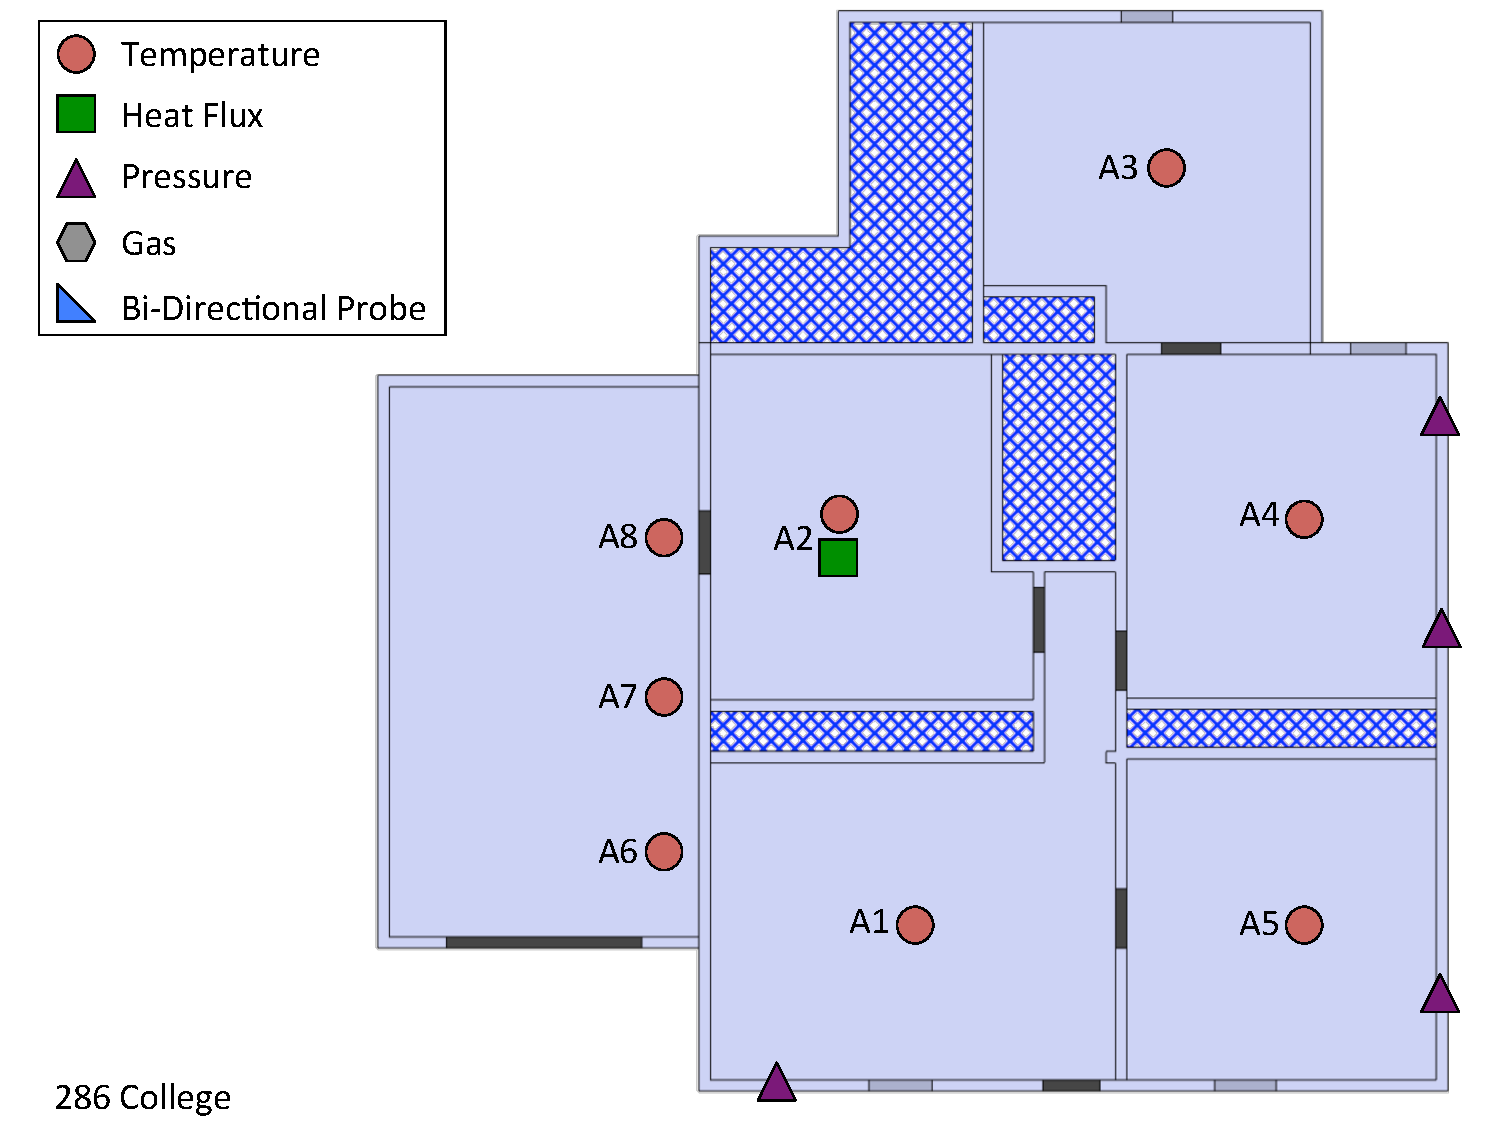
\includegraphics[width=6in]{../Figures/Instrumentation/286_College}
\caption{Instrumentation, 286 College}
\label{fig:Instrumentation_286_College}
\end{figure}

\begin{figure}[!ht]
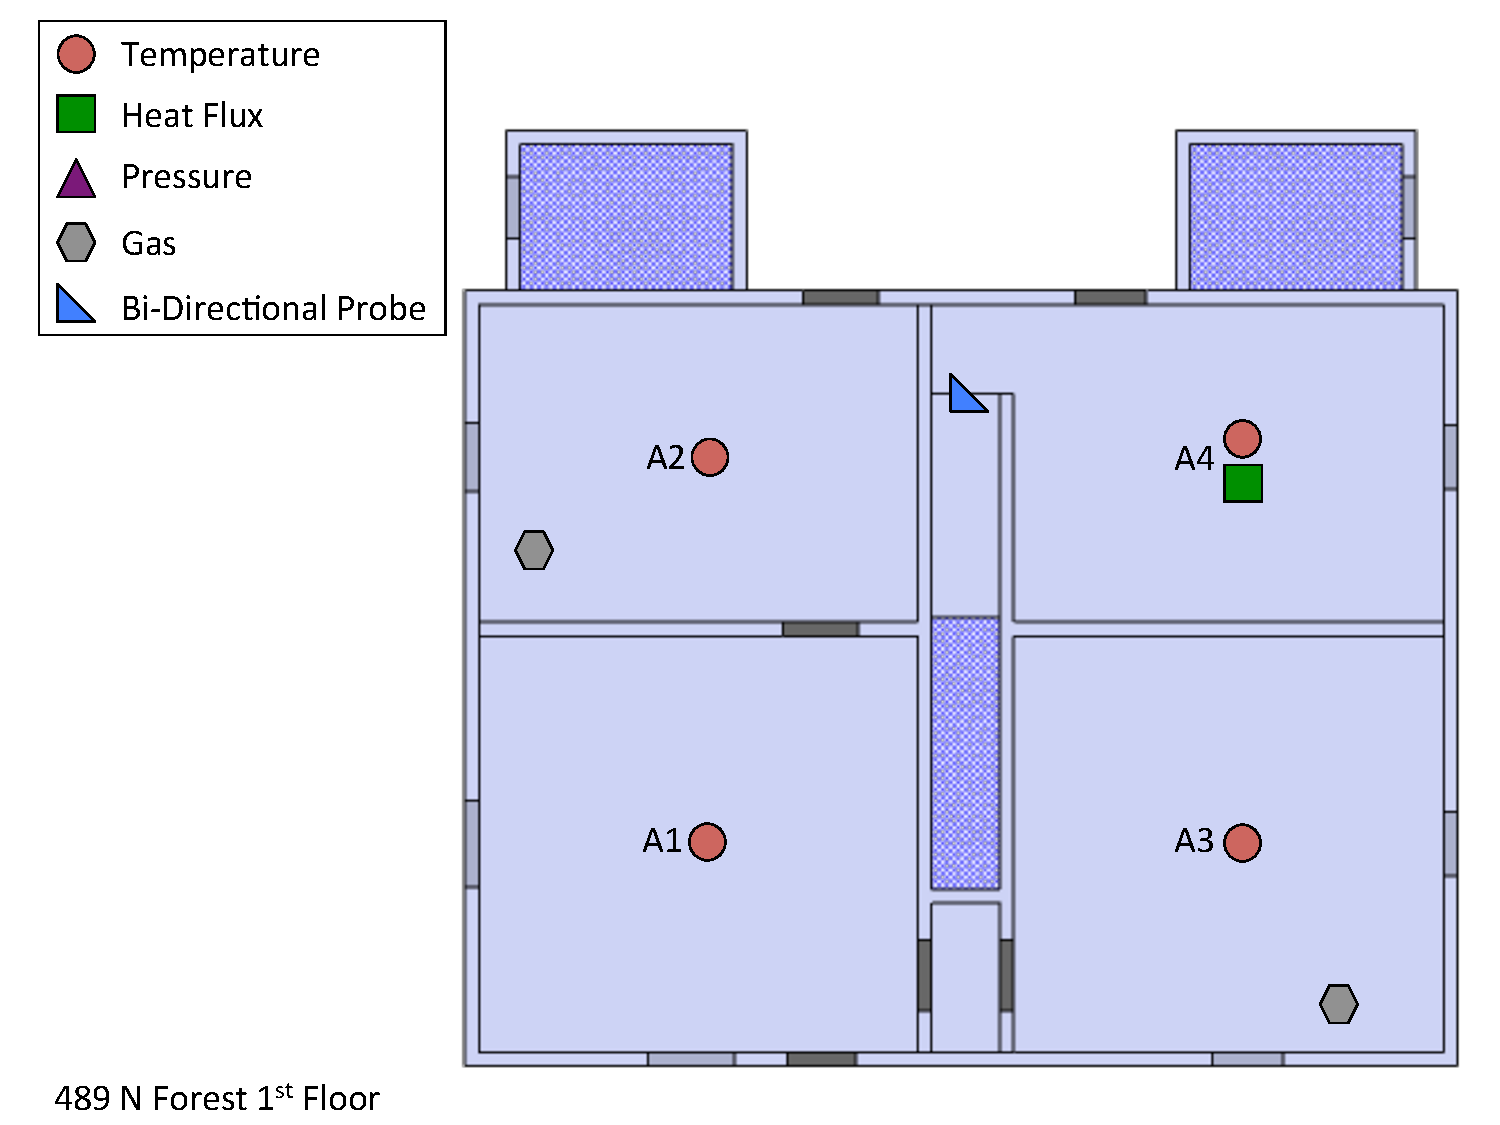
\includegraphics[width=6in]{../Figures/Instrumentation/489_N_Forest_1st_Floor}
\caption{Instrumentation, 489 N. Forest, first floor}
\label{fig:Instrumentation_489_N_Forest_1st_Floor}
\end{figure}

\begin{figure}[!ht]
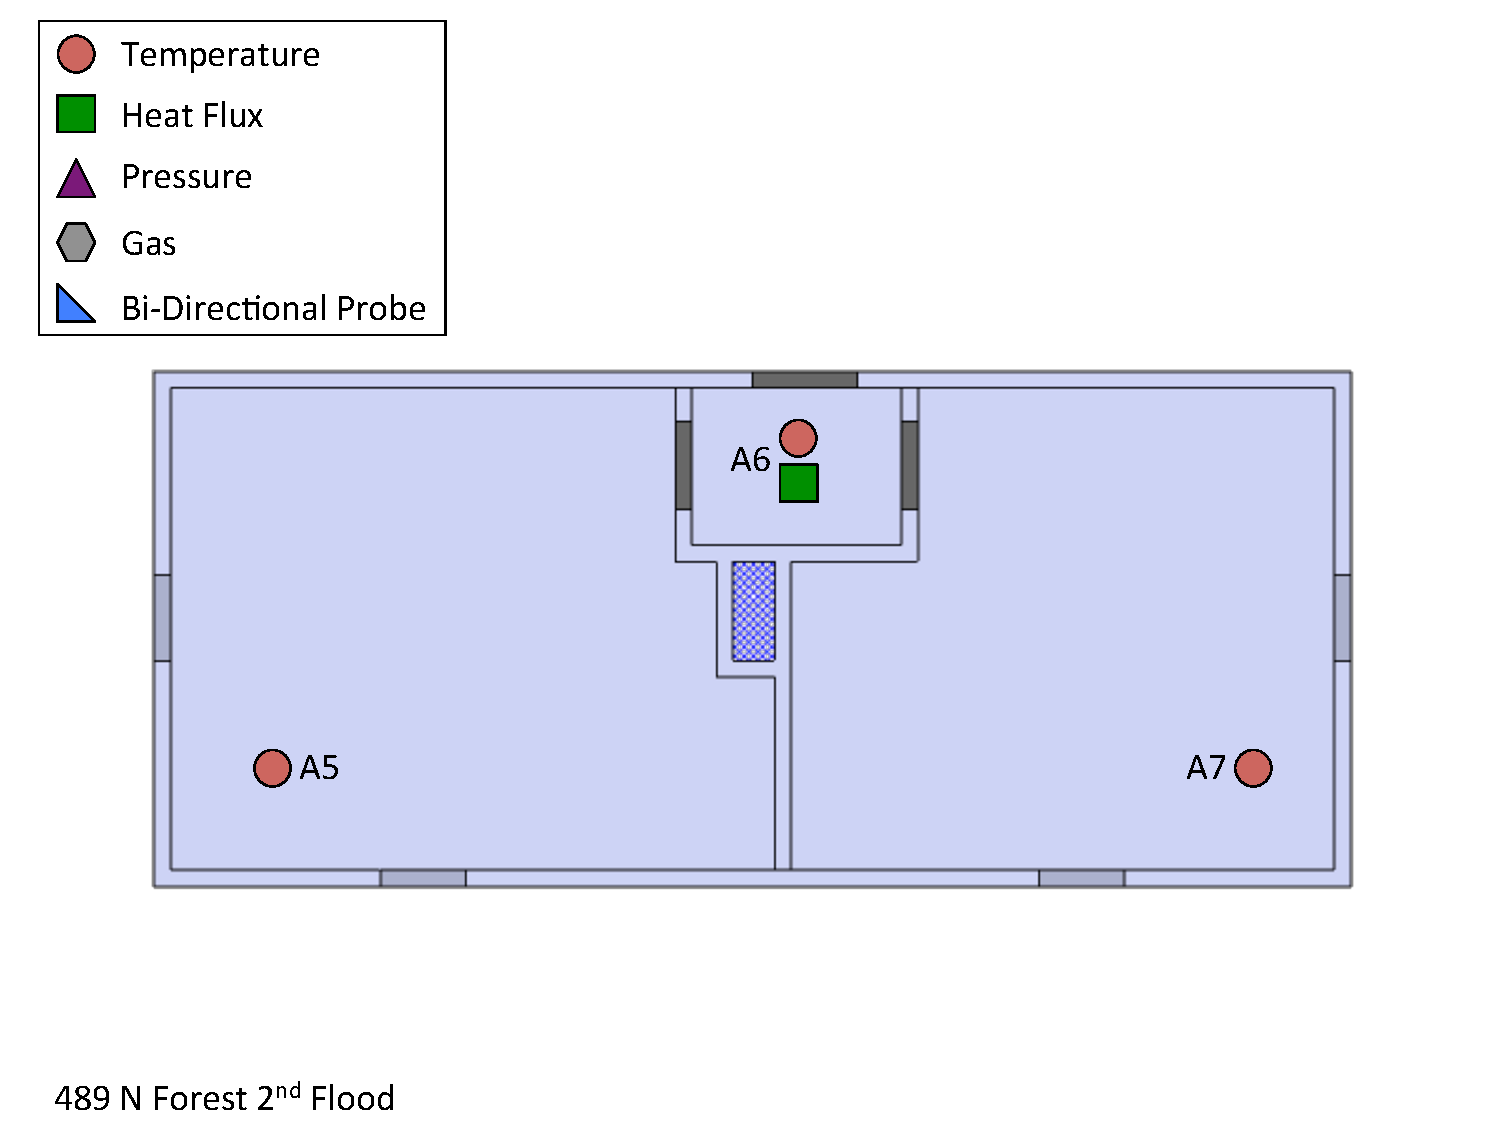
\includegraphics[width=6in]{../Figures/Instrumentation/489_N_Forest_2nd_Floor}
\caption{Instrumentation, 489 N. Forest, second floor}
\label{fig:Instrumentation_489_N_Forest_2nd_Floor}
\end{figure}

\begin{figure}[!ht]
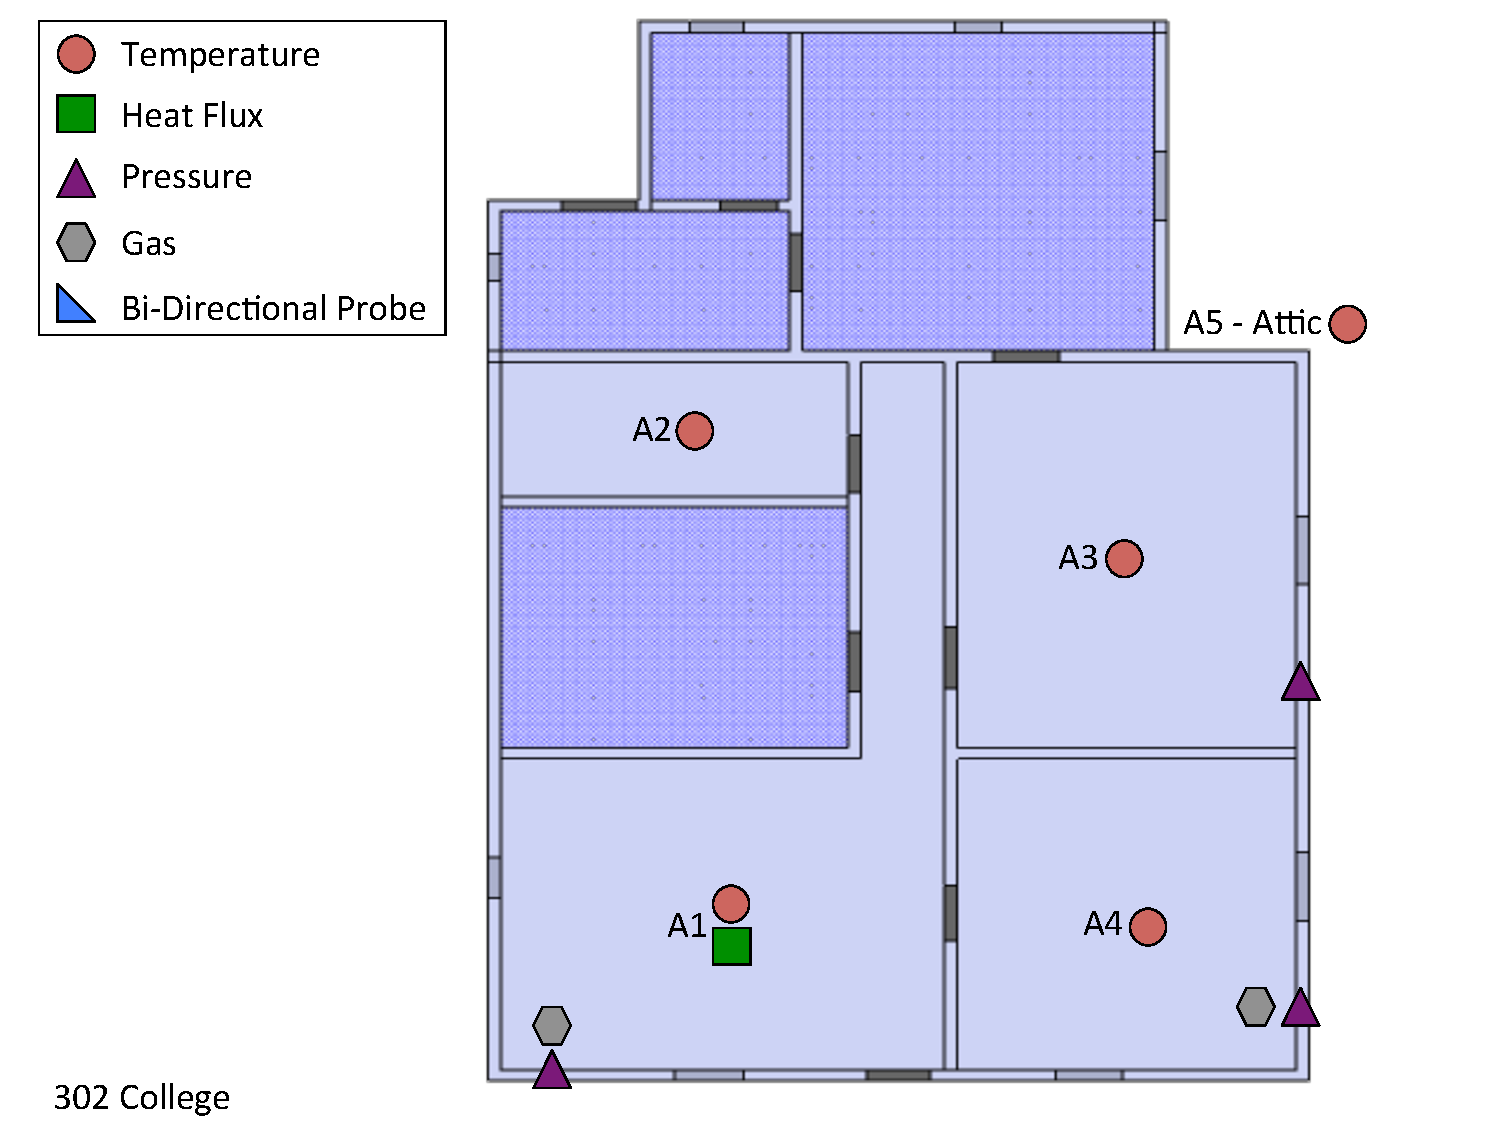
\includegraphics[width=6in]{../Figures/Instrumentation/302_College}
\caption{Instrumentation, 302 College}
\label{fig:Instrumentation_302_College}
\end{figure}

\begin{figure}[!ht]
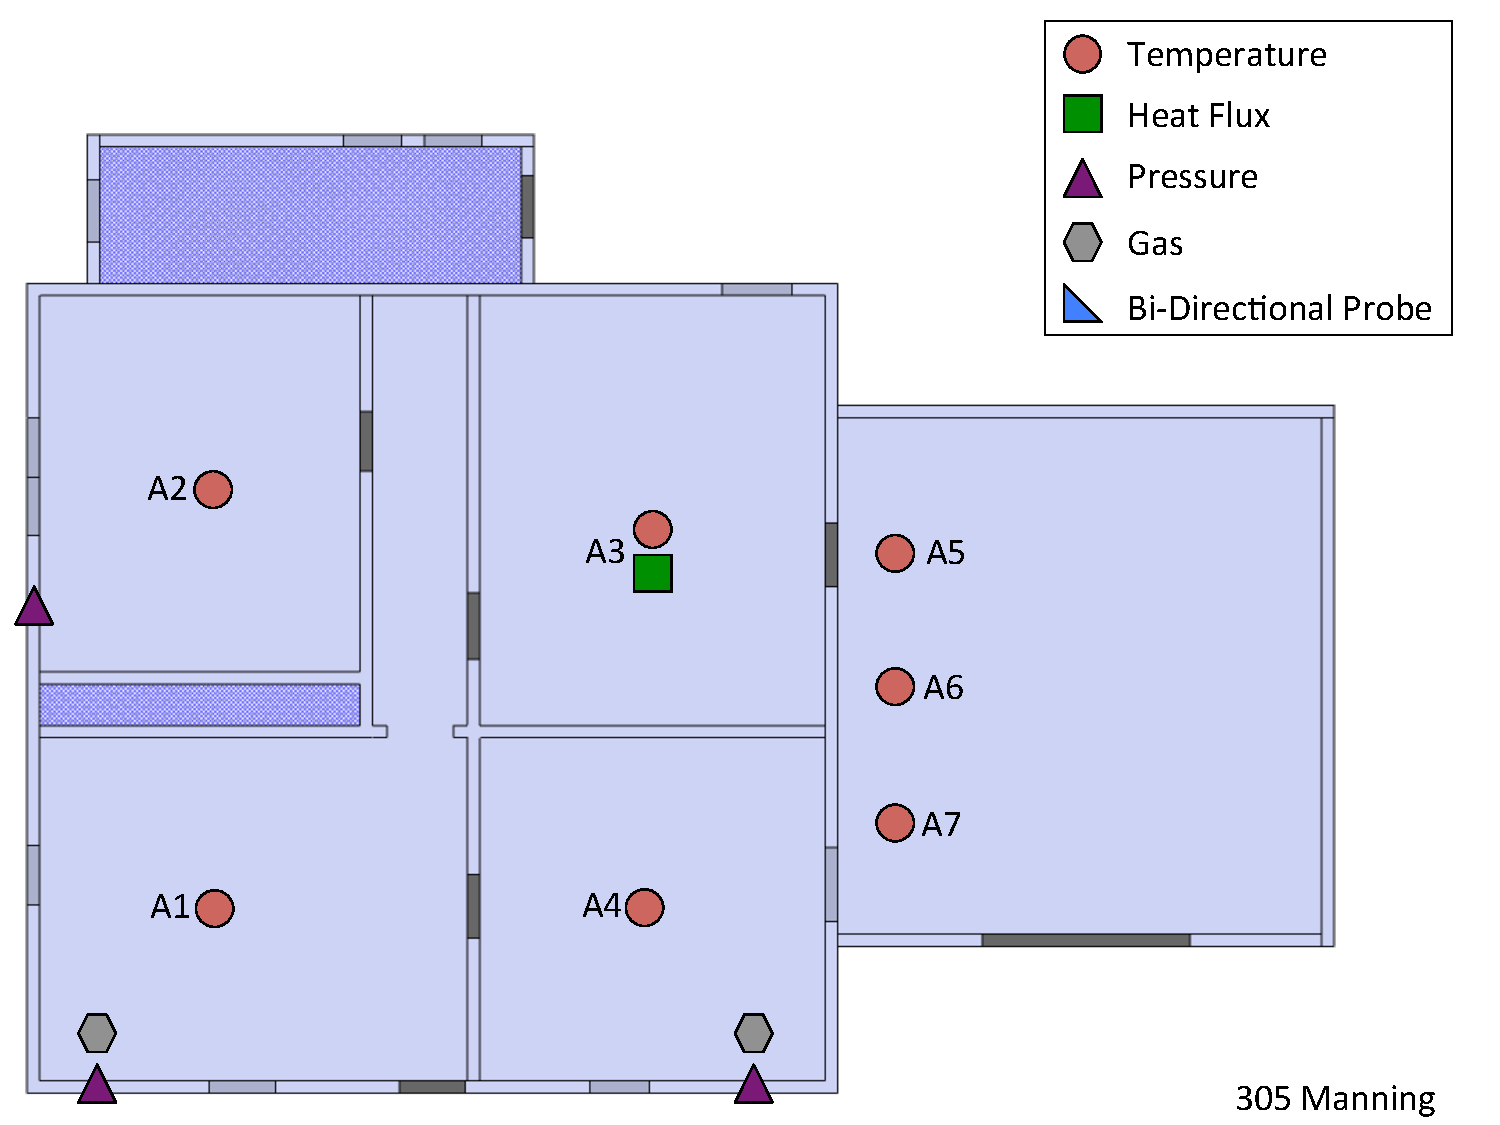
\includegraphics[width=6in]{../Figures/Instrumentation/305_Manning}
\caption{Instrumentation, 305 Manning}
\label{fig:Instrumentation_305_Manning}
\end{figure}

\begin{figure}[!ht]
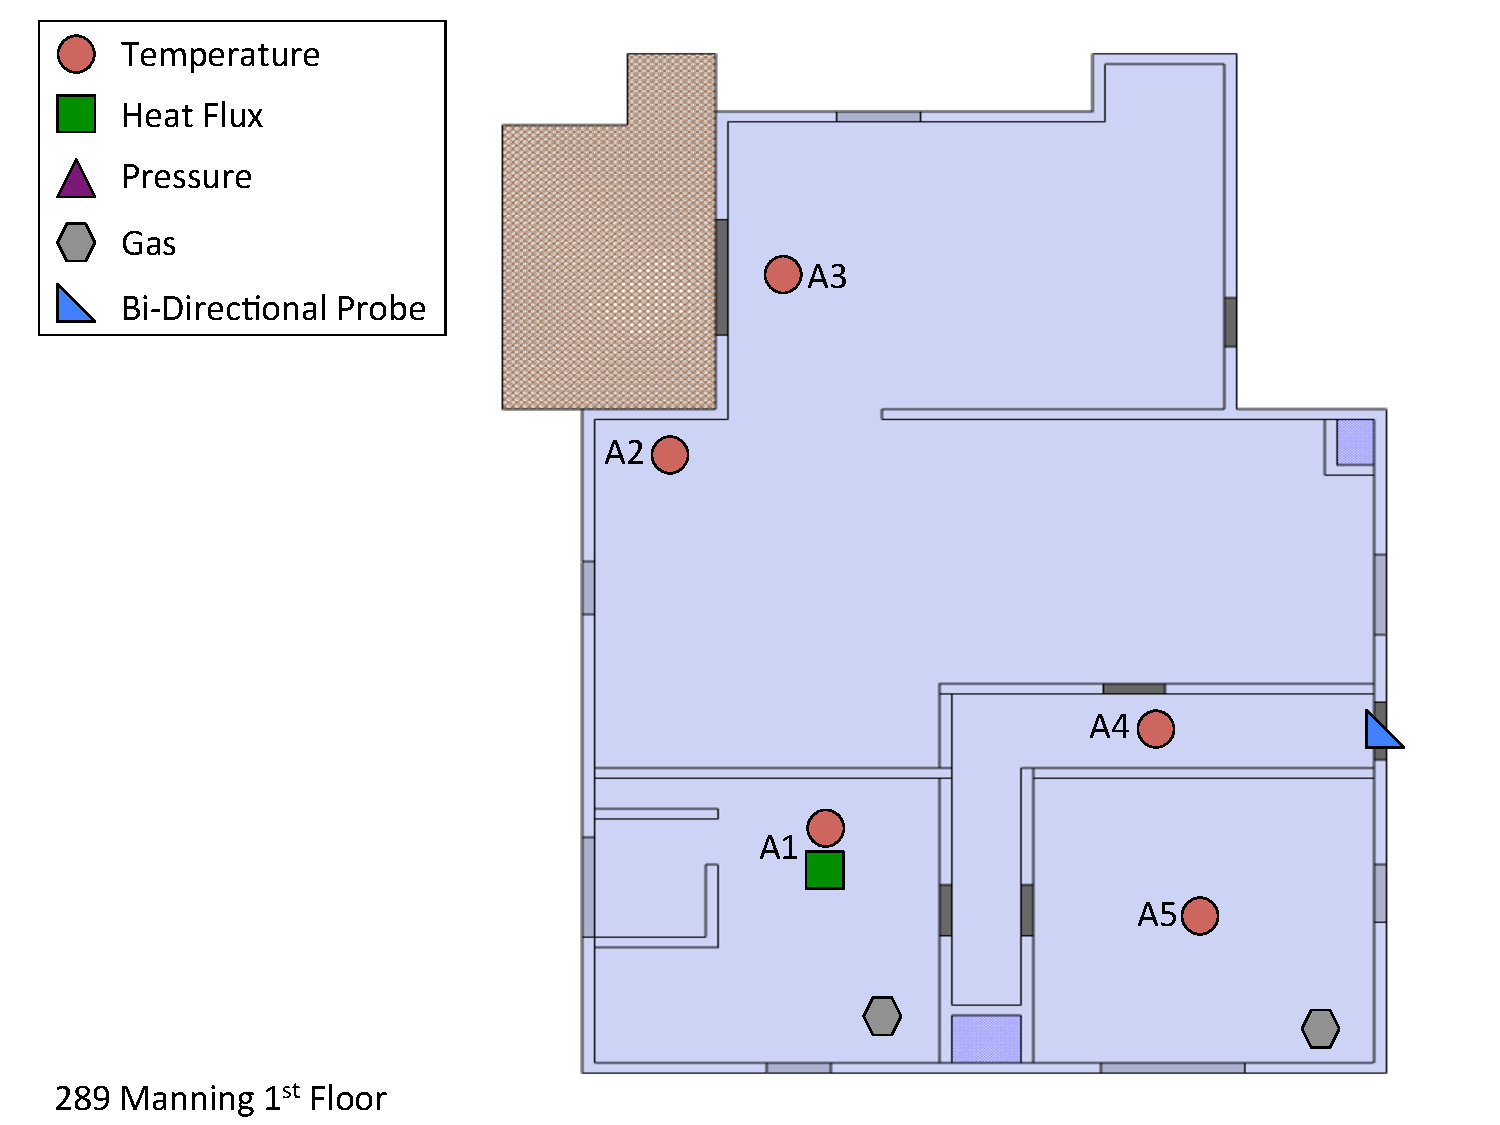
\includegraphics[width=6in]{../Figures/Instrumentation/289_Manning_1st_Floor}
\caption{Instrumentation, 289 Manning, first floor}
\label{fig:Instrumentation_289_Manning_1st_Floor}
\end{figure}

\begin{figure}[!ht]
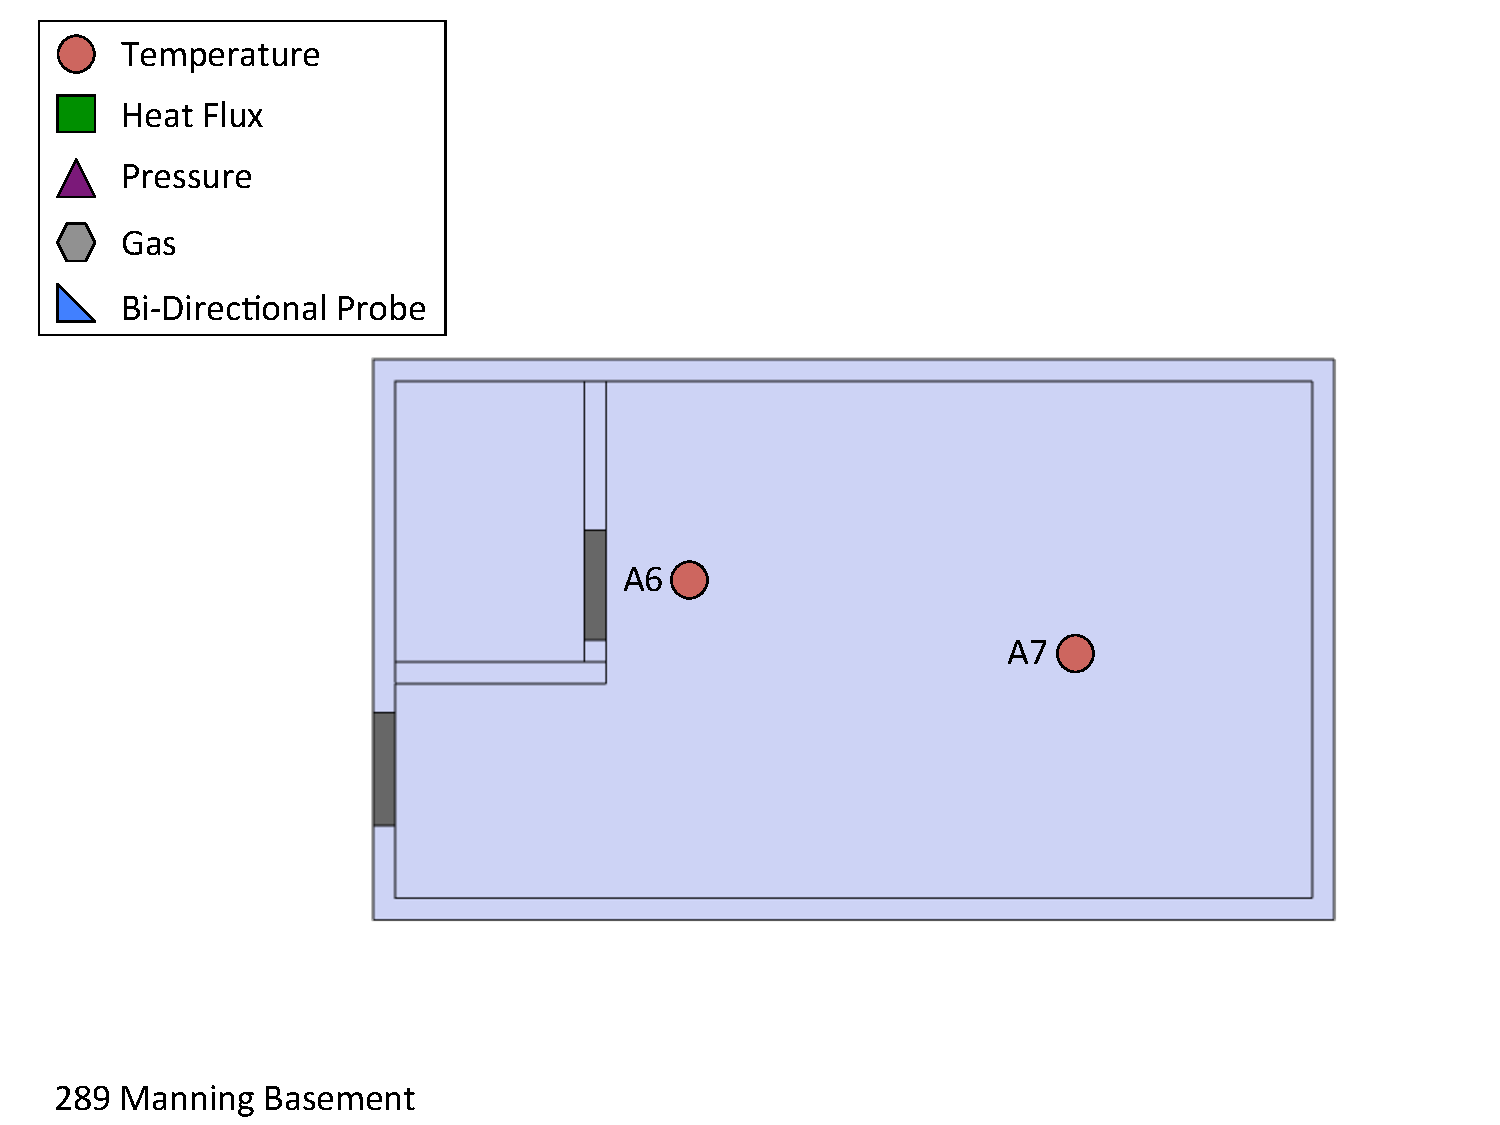
\includegraphics[width=6in]{../Figures/Instrumentation/289_Manning_Basement}
\caption{Instrumentation, 289 Manning, basement}
\label{fig:Instrumentation_289_Manning_basement}
\end{figure}


\clearpage


\section{Fuel Load}
\label{sec:Fuel_Load}

\begin{sidewaystable}[!ht]
\centering
\caption{Fuel masses}
\begin{tabular}{llcc}
\hline\noalign{\smallskip}
Item                         &  Material Description             &  Dimensions (m)            &  Mass (kg)  \\
\noalign{\smallskip}\hline\noalign{\smallskip}
% 3-seat Legacy Sofa         &  491 Brawley                      &  1.96 m x 0.86 m x 0.89 m  &  56.2 kg    \\
%   Cushion (left)           &  Cotton w/ inner springs          &                            &  4.06 kg    \\
%   Cushions (center)        &  Cotton w/ inner springs          &                            &  4.56 kg    \\
%   Cushions (rear)          &  Cotton w/ inner springs          &                            &  4.16 kg    \\
% 2-seat New Sofa            &  491 Brawley                      &  1.59 m x 0.91 m x 0.86 m  &  33.3 kg    \\
%   Cushion (seat)           &                                   &  0.56 m x 0.61 m x 0.14 m  &  1.6 kg     \\
%   Cushion (rear)           &  0.71 m at top, 0.58 m at bottom  &  Varies x 0.53 m x 0.20 m  &  2.0 kg     \\
3-seat Brown Sofa            &  302 College (front room)         &  2.24 m x 1.02 m x 0.91 m  &  61.0 kg    \\
2-seat Purple Stripe Sofa    &  302 College (front room)         &  1.57 m x 0.97 m x 0.86 m  &  82.0 kg    \\
3-seat Black Pine Leaf Sofa  &  302 College (front room)         &  2.08 m x 0.86 m x 0.86 m  &  51.0 kg    \\
Blue/Brown Chair             &  302 College (front room)         &  0.97 m x 0.81 m x 0.97 m  &  46.4 kg    \\
2-seat Floral Sofa           &  302 College (rear room)          &  1.68 m x 0.91 m x 0.91 m  &  34.5 kg    \\
2-seat Blue Plaid Sofa       &  302 College (rear room)          &  1.63 m x 0.97 m x 0.91 m  &  39.8 kg    \\
3-seat Yellow Sofa           &  302 College (rear room)          &  2.13 m x 0.91 m x 0.71 m  &  48.3 kg    \\
3-seat Floral Sofa           &  302 College (rear room)          &  2.29 m x 0.91 m x 0.91 m  &  48.0 kg    \\
3-seat New Sofa              &  289 College (front room)         &  2.13 m x 0.91 m x 0.91 m  &  43.0 kg    \\
Blue Chair                   &  289 College (middle room)        &  0.91 m x 0.91 m x 0.91 m  &  25.3 kg    \\
3-seat Floral Sofa           &  289 College (sprinkler room)     &  2.24 m x 1.02 m x 1.02 m  &  81.2 kg    \\
Floral Chair                 &  289 College (sprinkler room)     &  1.02 m x 1.02 m x 1.02 m  &  36.3 kg    \\
\noalign{\smallskip}\hline
\end{tabular}
\label{tab:Fuel_Masses}
\end{sidewaystable}

\chapter{Results}
\label{chap:Results}


\clearpage


\chapter{Conclusions}
\label{chap:Conclusions}

\chapter{Acknowledgments}
\label{chap:Acknowledgments}

\bibliography{../../../Bibliography/FDS_refs,../../../Bibliography/FDS_general,references}

\appendix

\chapter{All Tests}

\section{286 College}

\subsection{Test 1, Living room fire with sprinkler}

\begin{figure}[!ht]
\includegraphics[width=5in]{../Figures/Script_Figures/286_College_Test_1_TC_A3}
\caption{286 College, Test 1, Temperature TC\_A3}
\label{fig:286_College_Test_1_TC_A3}
\end{figure}

\begin{figure}[!ht]
\includegraphics[width=5in]{../Figures/Script_Figures/286_College_Test_1_TC_A4}
\caption{286 College, Test 1, Temperature TC\_A4}
\label{fig:286_College_Test_1_TC_A4}
\end{figure}

\begin{figure}[!ht]
\includegraphics[width=5in]{../Figures/Script_Figures/286_College_Test_1_TC_S_1}
\caption{286 College, Test 1, Temperature TC\_S\_1}
\label{fig:286_College_Test_1_TC_S_1}
\end{figure}


\clearpage


\subsection{Test 2, Garage fire, exterior attack}

\begin{figure}[!ht]
\includegraphics[width=5in]{../Figures/Script_Figures/286_College_Test_2_TC_A1}
\caption{286 College, Test 2, Temperature TC\_A1}
\label{fig:286_College_Test_2_TC_A1}
\end{figure}

\begin{figure}[!ht]
\includegraphics[width=5in]{../Figures/Script_Figures/286_College_Test_2_TC_A2}
\caption{286 College, Test 2, Temperature TC\_A2}
\label{fig:286_College_Test_2_TC_A2}
\end{figure}

\begin{figure}[!ht]
\includegraphics[width=5in]{../Figures/Script_Figures/286_College_Test_2_TC_A6}
\caption{286 College, Test 2, Temperature TC\_A6}
\label{fig:286_College_Test_2_TC_A6}
\end{figure}

\begin{figure}[!ht]
\includegraphics[width=5in]{../Figures/Script_Figures/286_College_Test_2_TC_A7}
\caption{286 College, Test 2, Temperature TC\_A7}
\label{fig:286_College_Test_2_TC_A7}
\end{figure}

\begin{figure}[!ht]
\includegraphics[width=5in]{../Figures/Script_Figures/286_College_Test_2_TC_A8}
\caption{286 College, Test 2, Temperature TC\_A8}
\label{fig:286_College_Test_2_TC_A8}
\end{figure}

\begin{figure}[!ht]
\includegraphics[width=5in]{../Figures/Script_Figures/286_College_Test_2_HF}
\caption{286 College, Test 2, Heat Flux}
\label{fig:286_College_Test_2_HF}
\end{figure}

\begin{figure}[!ht]
\includegraphics[width=5in]{../Figures/Script_Figures/286_College_Test_2_P_S_1}
\caption{286 College, Test 2, Pressure}
\label{fig:286_College_Test_2_P_S_1}
\end{figure}


\clearpage


\subsection{Test 3, Living room fire}

\begin{figure}[!ht]
\includegraphics[width=5in]{../Figures/Script_Figures/286_College_Test_3_TC_A1}
\caption{286 College, Test 3, Temperature TC\_A1}
\label{fig:286_College_Test_3_TC_A1}
\end{figure}

\begin{figure}[!ht]
\includegraphics[width=5in]{../Figures/Script_Figures/286_College_Test_3_TC_A4}
\caption{286 College, Test 3, Temperature TC\_A4}
\label{fig:286_College_Test_3_TC_A4}
\end{figure}

\begin{figure}[!ht]
\includegraphics[width=5in]{../Figures/Script_Figures/286_College_Test_3_TC_A5}
\caption{286 College, Test 3, Temperature TC\_A5}
\label{fig:286_College_Test_3_TC_A5}
\end{figure}

\begin{figure}[!ht]
\includegraphics[width=5in]{../Figures/Script_Figures/286_College_Test_3_HF}
\caption{286 College, Test 3, Heat Flux}
\label{fig:286_College_Test_3_HF}
\end{figure}

\begin{figure}[!ht]
\includegraphics[width=5in]{../Figures/Script_Figures/286_College_Test_3_P_S_1}
\caption{286 College, Test 3, Pressure}
\label{fig:286_College_Test_3_P_S_1}
\end{figure}


\clearpage


\section{489 N. Forest}

\subsection{Test 1, Living room fire}

\begin{figure}[!ht]
\includegraphics[width=5in]{../Figures/Script_Figures/489_N_Forest_Test_1_TC_A1}
\caption{489 N. Forest, Test 1, Temperature TC\_A1}
\label{fig:489_N_Forest_Test_1_TC_A1}
\end{figure}

\begin{figure}[!ht]
\includegraphics[width=5in]{../Figures/Script_Figures/489_N_Forest_Test_1_TC_A2}
\caption{489 N. Forest, Test 1, Temperature TC\_A2}
\label{fig:489_N_Forest_Test_1_TC_A2}
\end{figure}

\begin{figure}[!ht]
\includegraphics[width=5in]{../Figures/Script_Figures/489_N_Forest_Test_1_TC_A3}
\caption{489 N. Forest, Test 1, Temperature TC\_A3}
\label{fig:489_N_Forest_Test_1_TC_A3}
\end{figure}

\begin{figure}[!ht]
\includegraphics[width=5in]{../Figures/Script_Figures/489_N_Forest_Test_1_TC_S_1}
\caption{489 N. Forest, Test 1, Temperature TC\_S\_1}
\label{fig:489_N_Forest_Test_1_TC_S_1}
\end{figure}

\begin{figure}[!ht]
\includegraphics[width=5in]{../Figures/Script_Figures/489_N_Forest_Test_1_HF}
\caption{489 N. Forest, Test 1, Heat Flux}
\label{fig:489_N_Forest_Test_1_HF}
\end{figure}

\begin{figure}[!ht]
\includegraphics[width=5in]{../Figures/Script_Figures/489_N_Forest_Test_1_P_S_1}
\caption{489 N. Forest, Test 1, Pressure}
\label{fig:489_N_Forest_Test_1_P_S_1}
\end{figure}

\begin{figure}[!ht]
\includegraphics[width=5in]{../Figures/Script_Figures/489_N_Forest_Test_1_GAS}
\caption{489 N. Forest, Test 1, Gas Concentration}
\label{fig:489_N_Forest_Test_1_GAS}
\end{figure}


\clearpage


\subsection{Test 2, Second floor bedroom fire}

\begin{figure}[!ht]
\includegraphics[width=5in]{../Figures/Script_Figures/489_N_Forest_Test_2_TC_A4}
\caption{489 N. Forest, Test 2, Temperature TC\_A4}
\label{fig:489_N_Forest_Test_2_TC_A4}
\end{figure}

\begin{figure}[!ht]
\includegraphics[width=5in]{../Figures/Script_Figures/489_N_Forest_Test_2_TC_A5}
\caption{489 N. Forest, Test 2, Temperature TC\_A5}
\label{fig:489_N_Forest_Test_2_TC_A5}
\end{figure}

\begin{figure}[!ht]
\includegraphics[width=5in]{../Figures/Script_Figures/489_N_Forest_Test_2_TC_A6}
\caption{489 N. Forest, Test 2, Temperature TC\_A6}
\label{fig:489_N_Forest_Test_2_TC_A6}
\end{figure}

\begin{figure}[!ht]
\includegraphics[width=5in]{../Figures/Script_Figures/489_N_Forest_Test_2_TC_A7}
\caption{489 N. Forest, Test 2, Temperature TC\_A7}
\label{fig:489_N_Forest_Test_2_TC_A7}
\end{figure}

\begin{figure}[!ht]
\includegraphics[width=5in]{../Figures/Script_Figures/489_N_Forest_Test_2_TC_S_1}
\caption{489 N. Forest, Test 2, Temperature TC\_S\_1}
\label{fig:489_N_Forest_Test_2_TC_S_1}
\end{figure}

\begin{figure}[!ht]
\includegraphics[width=5in]{../Figures/Script_Figures/489_N_Forest_Test_2_HF}
\caption{489 N. Forest, Test 2, Heat Flux}
\label{fig:489_N_Forest_Test_2_HF}
\end{figure}

\begin{figure}[!ht]
\includegraphics[width=5in]{../Figures/Script_Figures/489_N_Forest_Test_2_P_S_1}
\caption{489 N. Forest, Test 2, Pressure}
\label{fig:489_N_Forest_Test_2_P_S_1}
\end{figure}


\clearpage


\section{302 College}

\subsection{Test 1, Bedroom fire}

\begin{figure}[!ht]
\includegraphics[width=5in]{../Figures/Script_Figures/302_College_Test_1_TC_A1}
\caption{302 College, Test 1, Temperature TC\_A1}
\label{fig:302_College_Test_1_TC_A1}
\end{figure}

\begin{figure}[!ht]
\includegraphics[width=5in]{../Figures/Script_Figures/302_College_Test_1_TC_A3}
\caption{302 College, Test 1, Temperature TC\_A3}
\label{fig:302_College_Test_1_TC_A3}
\end{figure}

\begin{figure}[!ht]
\includegraphics[width=5in]{../Figures/Script_Figures/302_College_Test_1_TC_A4}
\caption{302 College, Test 1, Temperature TC\_A4}
\label{fig:302_College_Test_1_TC_A4}
\end{figure}

\begin{figure}[!ht]
\includegraphics[width=5in]{../Figures/Script_Figures/302_College_Test_1_TC_A5}
\caption{302 College, Test 1, Temperature TC\_A5}
\label{fig:302_College_Test_1_TC_A5}
\end{figure}

\begin{figure}[!ht]
\includegraphics[width=5in]{../Figures/Script_Figures/302_College_Test_1_TC_S_1}
\caption{302 College, Test 1, Temperature TC\_S\_1}
\label{fig:302_College_Test_1_TC_S_1}
\end{figure}

\begin{figure}[!ht]
\includegraphics[width=5in]{../Figures/Script_Figures/302_College_Test_1_HF}
\caption{302 College, Test 1, Heat Flux}
\label{fig:302_College_Test_1_HF}
\end{figure}

\begin{figure}[!ht]
\includegraphics[width=5in]{../Figures/Script_Figures/302_College_Test_1_P_S_1}
\caption{302 College, Test 1, Pressure}
\label{fig:302_College_Test_1_P_S_1}
\end{figure}

\begin{figure}[!ht]
\includegraphics[width=5in]{../Figures/Script_Figures/302_College_Test_1_GAS}
\caption{302 College, Test 1, Gas Concentration}
\label{fig:302_College_Test_1_GAS}
\end{figure}


\clearpage


\subsection{Test 2, Living room fire}

\begin{figure}[!ht]
\includegraphics[width=5in]{../Figures/Script_Figures/302_College_Test_2_TC_A1}
\caption{302 College, Test 2, Temperature TC\_A1}
\label{fig:302_College_Test_2_TC_A1}
\end{figure}

\begin{figure}[!ht]
\includegraphics[width=5in]{../Figures/Script_Figures/302_College_Test_2_TC_A3}
\caption{302 College, Test 2, Temperature TC\_A3}
\label{fig:302_College_Test_2_TC_A3}
\end{figure}

\begin{figure}[!ht]
\includegraphics[width=5in]{../Figures/Script_Figures/302_College_Test_2_TC_A4}
\caption{302 College, Test 2, Temperature TC\_A4}
\label{fig:302_College_Test_2_TC_A4}
\end{figure}

\begin{figure}[!ht]
\includegraphics[width=5in]{../Figures/Script_Figures/302_College_Test_2_TC_A5}
\caption{302 College, Test 2, Temperature TC\_A5}
\label{fig:302_College_Test_2_TC_A5}
\end{figure}

\begin{figure}[!ht]
\includegraphics[width=5in]{../Figures/Script_Figures/302_College_Test_2_TC_S_1}
\caption{302 College, Test 2, Temperature TC\_S\_1}
\label{fig:302_College_Test_2_TC_S_1}
\end{figure}

\begin{figure}[!ht]
\includegraphics[width=5in]{../Figures/Script_Figures/302_College_Test_2_HF}
\caption{302 College, Test 2, Heat Flux}
\label{fig:302_College_Test_2_HF}
\end{figure}

\begin{figure}[!ht]
\includegraphics[width=5in]{../Figures/Script_Figures/302_College_Test_2_P_S_1}
\caption{302 College, Test 2, Pressure}
\label{fig:302_College_Test_2_P_S_1}
\end{figure}

\begin{figure}[!ht]
\includegraphics[width=5in]{../Figures/Script_Figures/302_College_Test_2_GAS}
\caption{302 College, Test 2, Gas Concentration}
\label{fig:302_College_Test_2_GAS}
\end{figure}


\clearpage


\subsection{Test 3, Bathroom and attic fire}

\begin{figure}[!ht]
\includegraphics[width=5in]{../Figures/Script_Figures/302_College_Test_3_TC_A1}
\caption{302 College, Test 3, Temperature TC\_A1}
\label{fig:302_College_Test_3_TC_A1}
\end{figure}

\begin{figure}[!ht]
\includegraphics[width=5in]{../Figures/Script_Figures/302_College_Test_3_TC_A2}
\caption{302 College, Test 3, Temperature TC\_A2}
\label{fig:302_College_Test_3_TC_A2}
\end{figure}

\begin{figure}[!ht]
\includegraphics[width=5in]{../Figures/Script_Figures/302_College_Test_3_TC_A3}
\caption{302 College, Test 3, Temperature TC\_A3}
\label{fig:302_College_Test_3_TC_A3}
\end{figure}

\begin{figure}[!ht]
\includegraphics[width=5in]{../Figures/Script_Figures/302_College_Test_3_TC_A4}
\caption{302 College, Test 3, Temperature TC\_A4}
\label{fig:302_College_Test_3_TC_A4}
\end{figure}

\begin{figure}[!ht]
\includegraphics[width=5in]{../Figures/Script_Figures/302_College_Test_3_TC_A5}
\caption{302 College, Test 3, Temperature TC\_A5}
\label{fig:302_College_Test_3_TC_A5}
\end{figure}

\begin{figure}[!ht]
\includegraphics[width=5in]{../Figures/Script_Figures/302_College_Test_3_TC_S_1}
\caption{302 College, Test 3, Temperature TC\_S\_1}
\label{fig:302_College_Test_3_TC_S_1}
\end{figure}

\begin{figure}[!ht]
\includegraphics[width=5in]{../Figures/Script_Figures/302_College_Test_3_HF}
\caption{302 College, Test 3, Heat Flux}
\label{fig:302_College_Test_3_HF}
\end{figure}

\begin{figure}[!ht]
\includegraphics[width=5in]{../Figures/Script_Figures/302_College_Test_3_P_S_1}
\caption{302 College, Test 3, Pressure}
\label{fig:302_College_Test_3_P_S_1}
\end{figure}

\begin{figure}[!ht]
\includegraphics[width=5in]{../Figures/Script_Figures/302_College_Test_3_GAS}
\caption{302 College, Test 3, Gas Concentration}
\label{fig:302_College_Test_3_GAS}
\end{figure}


\clearpage


\section{305 Manning}

\subsection{Test 1, Garage fire, interior attack}

\begin{figure}[!ht]
\includegraphics[width=5in]{../Figures/Script_Figures/305_Manning_Test_1_TC_A1}
\caption{305 Manning, Test 1, Temperature TC\_A1}
\label{fig:305_Manning_Test_1_TC_A1}
\end{figure}

\begin{figure}[!ht]
\includegraphics[width=5in]{../Figures/Script_Figures/305_Manning_Test_1_TC_A2}
\caption{305 Manning, Test 1, Temperature TC\_A2}
\label{fig:305_Manning_Test_1_TC_A2}
\end{figure}

\begin{figure}[!ht]
\includegraphics[width=5in]{../Figures/Script_Figures/305_Manning_Test_1_TC_A3}
\caption{305 Manning, Test 1, Temperature TC\_A3}
\label{fig:305_Manning_Test_1_TC_A3}
\end{figure}

\begin{figure}[!ht]
\includegraphics[width=5in]{../Figures/Script_Figures/305_Manning_Test_1_TC_A4}
\caption{305 Manning, Test 1, Temperature TC\_A4}
\label{fig:305_Manning_Test_1_TC_A4}
\end{figure}

\begin{figure}[!ht]
\includegraphics[width=5in]{../Figures/Script_Figures/305_Manning_Test_1_TC_A5}
\caption{305 Manning, Test 1, Temperature TC\_A5}
\label{fig:305_Manning_Test_1_TC_A5}
\end{figure}

\begin{figure}[!ht]
\includegraphics[width=5in]{../Figures/Script_Figures/305_Manning_Test_1_TC_A6}
\caption{305 Manning, Test 1, Temperature TC\_A6}
\label{fig:305_Manning_Test_1_TC_A6}
\end{figure}

\begin{figure}[!ht]
\includegraphics[width=5in]{../Figures/Script_Figures/305_Manning_Test_1_TC_A7}
\caption{305 Manning, Test 1, Temperature TC\_A7}
\label{fig:305_Manning_Test_1_TC_A7}
\end{figure}

\begin{figure}[!ht]
\includegraphics[width=5in]{../Figures/Script_Figures/305_Manning_Test_1_HF}
\caption{305 Manning, Test 1, Heat Flux}
\label{fig:305_Manning_Test_1_HF}
\end{figure}

\begin{figure}[!ht]
\includegraphics[width=5in]{../Figures/Script_Figures/305_Manning_Test_1_P_S_1}
\caption{305 Manning, Test 1, Pressure}
\label{fig:305_Manning_Test_1_P_S_1}
\end{figure}

\begin{figure}[!ht]
\includegraphics[width=5in]{../Figures/Script_Figures/305_Manning_Test_1_GAS}
\caption{305 Manning, Test 1, Gas Concentration}
\label{fig:305_Manning_Test_1_GAS}
\end{figure}


\clearpage


\subsection{Test 2, Bedroom fire}

\begin{figure}[!ht]
\includegraphics[width=5in]{../Figures/Script_Figures/305_Manning_Test_2_TC_A1}
\caption{305 Manning, Test 2, Temperature TC\_A1}
\label{fig:305_Manning_Test_2_TC_A1}
\end{figure}

\begin{figure}[!ht]
\includegraphics[width=5in]{../Figures/Script_Figures/305_Manning_Test_2_TC_A2}
\caption{305 Manning, Test 2, Temperature TC\_A2}
\label{fig:305_Manning_Test_2_TC_A2}
\end{figure}

\begin{figure}[!ht]
\includegraphics[width=5in]{../Figures/Script_Figures/305_Manning_Test_2_TC_A3}
\caption{305 Manning, Test 2, Temperature TC\_A3}
\label{fig:305_Manning_Test_2_TC_A3}
\end{figure}

\begin{figure}[!ht]
\includegraphics[width=5in]{../Figures/Script_Figures/305_Manning_Test_2_TC_A4}
\caption{305 Manning, Test 2, Temperature TC\_A4}
\label{fig:305_Manning_Test_2_TC_A4}
\end{figure}

\begin{figure}[!ht]
\includegraphics[width=5in]{../Figures/Script_Figures/305_Manning_Test_2_TC_A5}
\caption{305 Manning, Test 2, Temperature TC\_A5}
\label{fig:305_Manning_Test_2_TC_A5}
\end{figure}

\begin{figure}[!ht]
\includegraphics[width=5in]{../Figures/Script_Figures/305_Manning_Test_2_TC_A6}
\caption{305 Manning, Test 2, Temperature TC\_A6}
\label{fig:305_Manning_Test_2_TC_A6}
\end{figure}

\begin{figure}[!ht]
\includegraphics[width=5in]{../Figures/Script_Figures/305_Manning_Test_2_TC_A7}
\caption{305 Manning, Test 2, Temperature TC\_A7}
\label{fig:305_Manning_Test_2_TC_A7}
\end{figure}

\begin{figure}[!ht]
\includegraphics[width=5in]{../Figures/Script_Figures/305_Manning_Test_2_TC_S_1}
\caption{305 Manning, Test 2, Temperature TC\_S\_1}
\label{fig:305_Manning_Test_2_TC_S_1}
\end{figure}

\begin{figure}[!ht]
\includegraphics[width=5in]{../Figures/Script_Figures/305_Manning_Test_2_HF}
\caption{305 Manning, Test 2, Heat Flux}
\label{fig:305_Manning_Test_2_HF}
\end{figure}

\begin{figure}[!ht]
\includegraphics[width=5in]{../Figures/Script_Figures/305_Manning_Test_2_P_S_1}
\caption{305 Manning, Test 2, Pressure}
\label{fig:305_Manning_Test_2_P_S_1}
\end{figure}

\begin{figure}[!ht]
\includegraphics[width=5in]{../Figures/Script_Figures/305_Manning_Test_2_GAS}
\caption{305 Manning, Test 2, Gas Concentration}
\label{fig:305_Manning_Test_2_GAS}
\end{figure}


% \clearpage

% Heat flux measurements are large negative values

% \subsection{Test 3, Complete burndown}

% \begin{figure}[!ht]
% \includegraphics[width=5in]{../Figures/Script_Figures/305_Manning_Test_3_HF}
% \caption{305 Manning, Test 3, Heat Flux}
% \label{fig:305_Manning_Test_3_HF}
% \end{figure}


\clearpage


\section{289 Manning}

\subsection{Test 1, Basement fire}

\begin{figure}[!ht]
\includegraphics[width=5in]{../Figures/Script_Figures/289_Manning_Test_1_TC_A1}
\caption{286 College, Test 1, Temperature TC\_A1}
\label{fig:289_Manning_Test_1_TC_A1}
\end{figure}

\begin{figure}[!ht]
\includegraphics[width=5in]{../Figures/Script_Figures/289_Manning_Test_1_TC_A4}
\caption{286 College, Test 1, Temperature TC\_A4}
\label{fig:289_Manning_Test_1_TC_A4}
\end{figure}

\begin{figure}[!ht]
\includegraphics[width=5in]{../Figures/Script_Figures/289_Manning_Test_1_TC_A5}
\caption{286 College, Test 1, Temperature TC\_A5}
\label{fig:289_Manning_Test_1_TC_A5}
\end{figure}

\begin{figure}[!ht]
\includegraphics[width=5in]{../Figures/Script_Figures/289_Manning_Test_1_TC_A6}
\caption{286 College, Test 1, Temperature TC\_A6}
\label{fig:289_Manning_Test_1_TC_A6}
\end{figure}

\begin{figure}[!ht]
\includegraphics[width=5in]{../Figures/Script_Figures/289_Manning_Test_1_TC_A7}
\caption{286 College, Test 1, Temperature TC\_A7}
\label{fig:289_Manning_Test_1_TC_A7}
\end{figure}

\begin{figure}[!ht]
\includegraphics[width=5in]{../Figures/Script_Figures/289_Manning_Test_1_TC_S_1}
\caption{286 College, Test 1, Temperature TC\_S\_1}
\label{fig:289_Manning_Test_1_TC_S_1}
\end{figure}

\begin{figure}[!ht]
\includegraphics[width=5in]{../Figures/Script_Figures/289_Manning_Test_1_HF}
\caption{286 College, Test 1, Heat Flux}
\label{fig:289_Manning_Test_1_HF}
\end{figure}

\begin{figure}[!ht]
\includegraphics[width=5in]{../Figures/Script_Figures/289_Manning_Test_1_P_S_1}
\caption{286 College, Test 1, Pressure}
\label{fig:289_Manning_Test_1_P_S_1}
\end{figure}

\begin{figure}[!ht]
\includegraphics[width=5in]{../Figures/Script_Figures/289_Manning_Test_1_GAS}
\caption{286 College, Test 1, Gas Concentration}
\label{fig:289_Manning_Test_1_GAS}
\end{figure}


\clearpage


\subsection{Test 2, Deck and attic fire}

\begin{figure}[!ht]
\includegraphics[width=5in]{../Figures/Script_Figures/289_Manning_Test_2_TC_A2}
\caption{286 College, Test 2, Temperature TC\_A2}
\label{fig:289_Manning_Test_2_TC_A2}
\end{figure}

\begin{figure}[!ht]
\includegraphics[width=5in]{../Figures/Script_Figures/289_Manning_Test_2_TC_A3}
\caption{286 College, Test 2, Temperature TC\_A3}
\label{fig:289_Manning_Test_2_TC_A3}
\end{figure}

\begin{figure}[!ht]
\includegraphics[width=5in]{../Figures/Script_Figures/289_Manning_Test_2_HF}
\caption{286 College, Test 2, Heat Flux}
\label{fig:289_Manning_Test_2_HF}
\end{figure}


\end{document}
